\chapter{Methodology}
Introduction goes here, no headline
train lottery tickets on simple task that contains independence.
The structure of lottery tickets is still mysterious. 
Analyzing the structure of a large and sparse Directed acyclic graph is not an easy task. 
However, one could approach the problem the other way around. 
Instead of analyzing the structure of an existing Lottery ticket, one could see what kind of structure appears given a problem with a known structure.
Inspired by the experiments in \autocite{BIMT}, a dataset that contains an independence problem was created.
The question is:
`Will a lottery ticket trained on an independece dataset result in seperate networks?'
In the course of this thesis, it is demonstrated that IMP indeed finds lottery tickets composed of two disconnected subnetworks inside a larger network.

\section{Software Stack}
All software developed within the scope of this thesis is written in python~\autocite{python}.
Several freely available python packages are used.
PyTorch~\autocite{pytorch}, a commonly used machine learning library, is used to define the neural networks and train them.
NetworkX~\autocite{networkx}, a well known library for working with mathematical graphs, is used to transform the pytorch model into a directed graph and analyse it.
Scikit-Learn~\autocite{sklearn} which is also a popular machine learning library, is used to generate the datasets.
Matplotlib~\autocite{matplotlib} is used to generate the plots to visualize the results of the experiments.
Numpy~\autocite{numpy}, a package to work with matrices in python, is used throughout this thesis to manipulate vectors and matrices.

\section{The Moons-Circles Dataset}\label{sec:independece_dataset}
\textcite{BIMT} executed the experiements on symbolic regression datasets.
These are simple toy datasets where the labels are computed with a symbolic formula. 
For instance regarding the independence task, the inputs are $x_1, x_2, x_3, x_4$ and the outputs are $y_1={x_2}^2 + \sin{(\pi*x_4)}$ and $y_2={(x_1+x_3)}^3$
In this case the independence is obvious, as $y_1$ depends only on $x_1$ and $x_3$, and $y_2$ depends only on $x_2$ and $x_4$.
However with regards to lottery tickets, the existing literature focuses on classification tasks, while this is a regression task.

Therefore instead of using the independence dataset from \autocite{BIMT}, a different dataset has to be created.

To create a simple toy classification task with independance, two classic toy datasets are concatenated into one dataset.

\begin{figure}[ht]
    \centering
    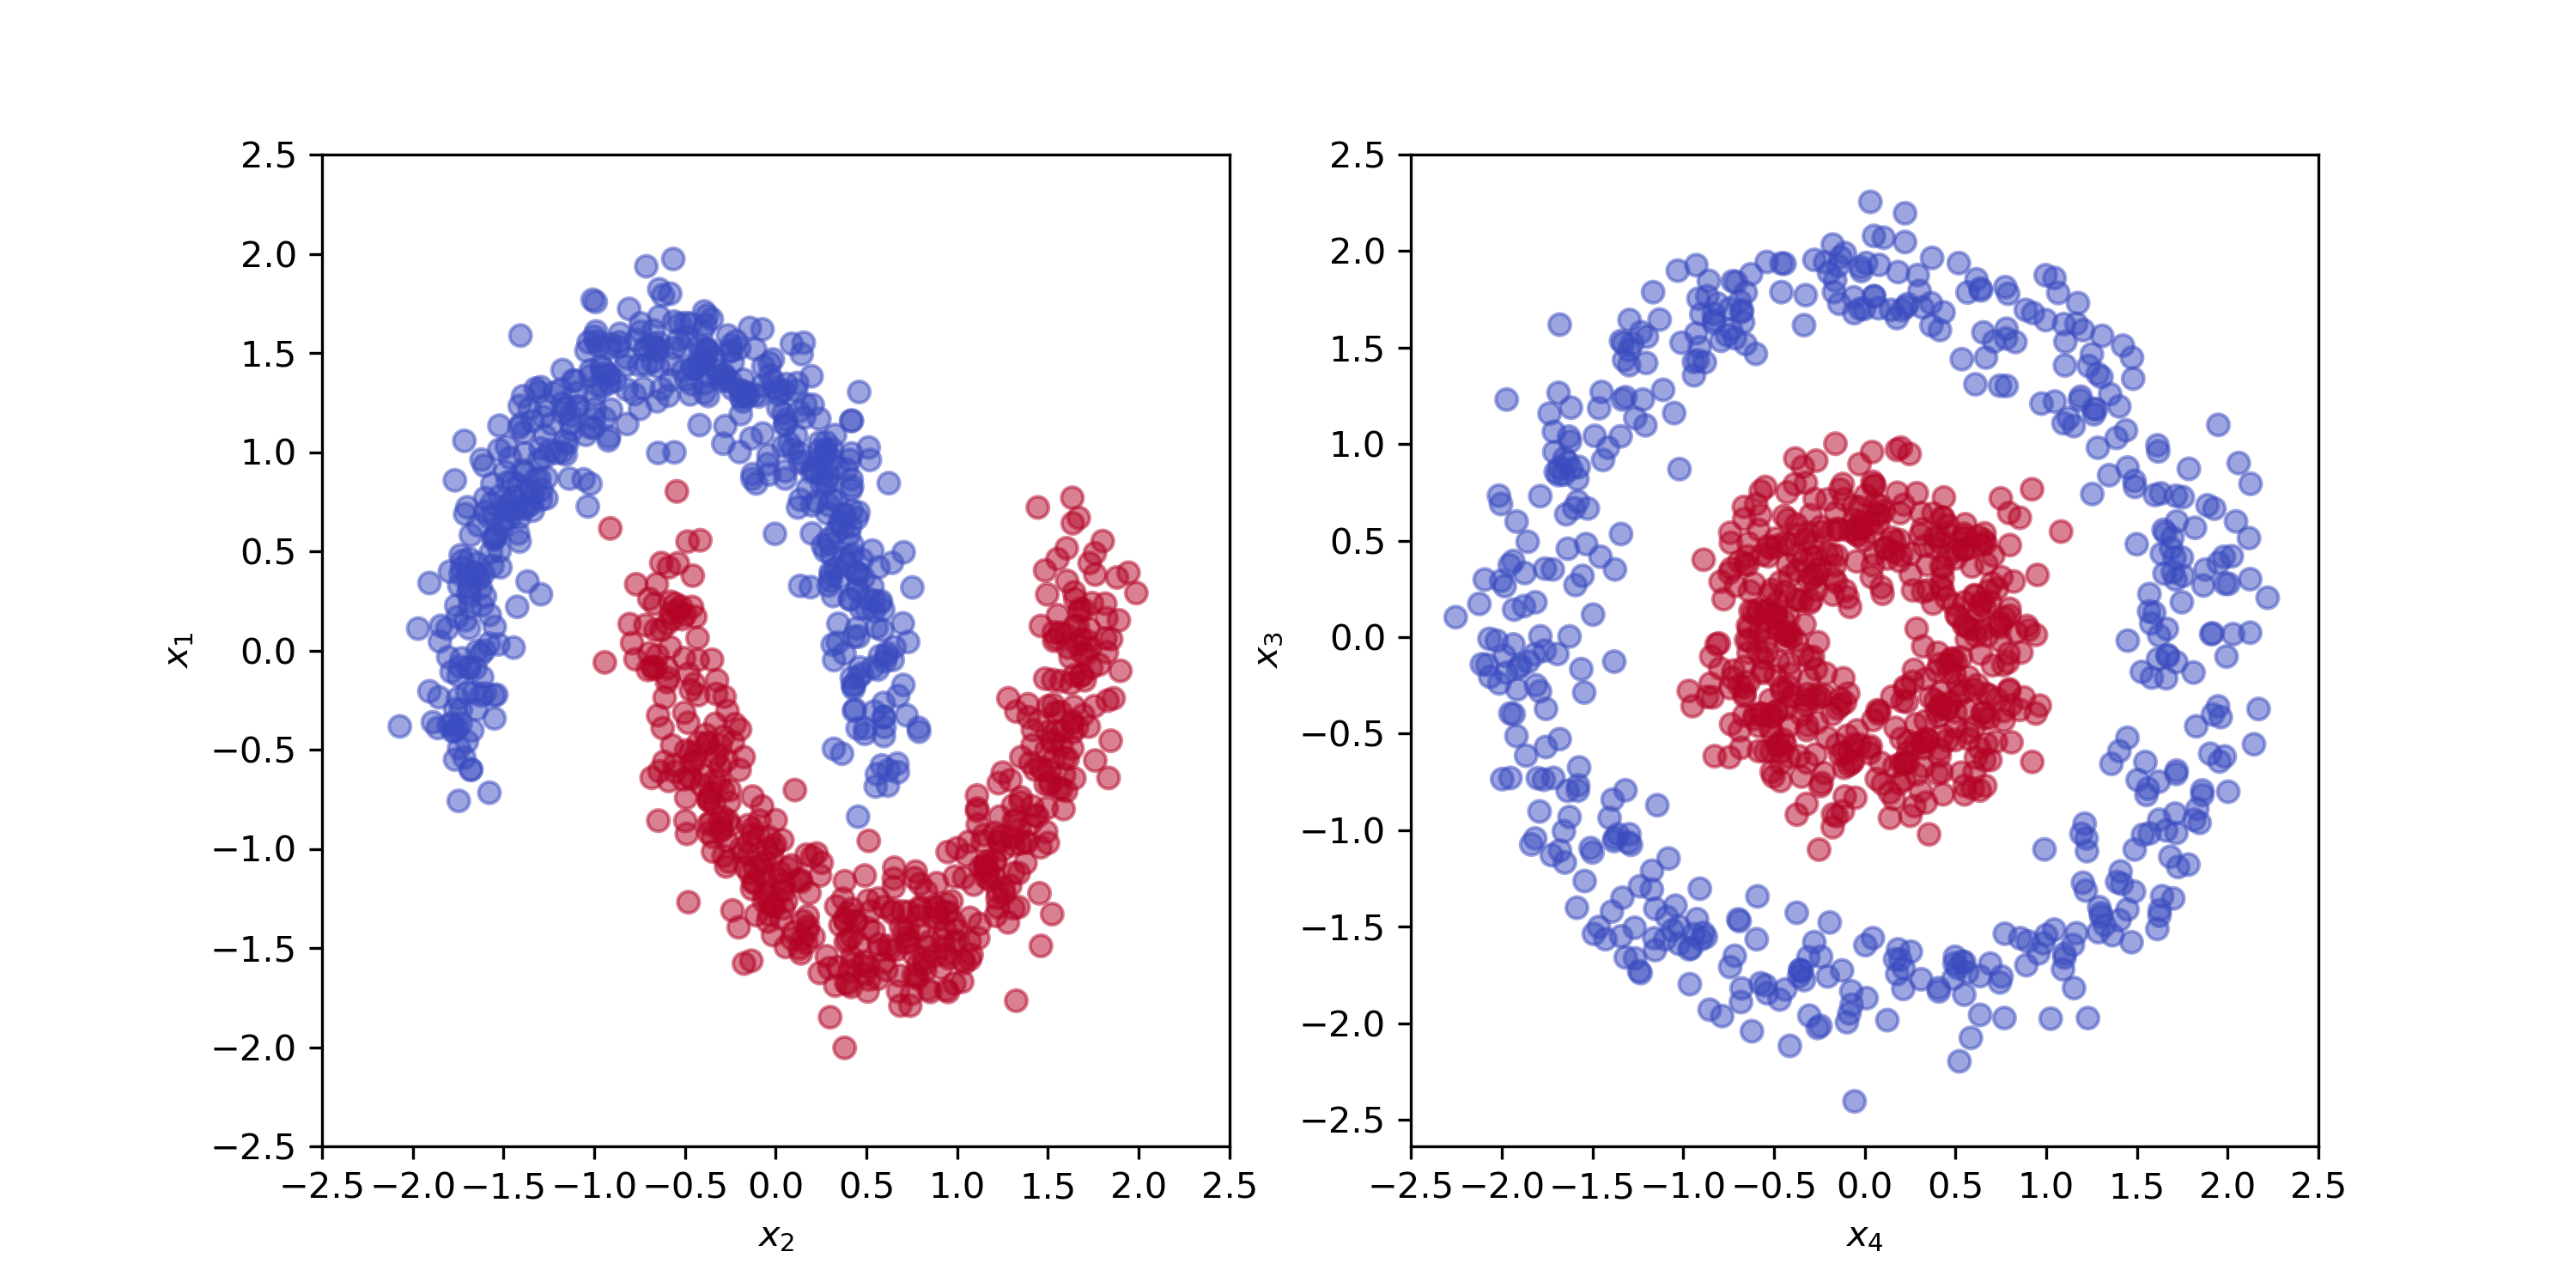
\includegraphics[width=1.0\linewidth]{moons-circles.png}
    \caption{
        This figure depicts the two dataset. 
        On the left, the `Two Moons Dataset' is displayed. 
        On the right, the `Circles' dataset. 
        The datasets are normalized to have zero mean and unit variance in each feature.
    }\label{fig:moons_circles}
\end{figure}

The two selected datasets are the two moons dataset and the Circles dataset, depicted in figure~\ref{fig:moons_circles}.

Both datasets can be interpreted as a two dimensional plane, where the inputs describe coordinates of points on the plane. 
The labels of the dataset relates to the class.
Each point belongs to one class: red or blue.
Concretley, let $\begin{pmatrix} x_1 & x_2 \end{pmatrix}$ be the inputs of the two-moons dataset and $y_1 \in \{0,1\}$ the class label.
The data is generated by creating two half circles of evently spaced points, with a radius of $1$.
One of the half circles is rotated by 180 degrees and shifted by $0.5$.
Gaussian noise with a mean of $0$ and standard deviation of $0.1$ is added to each point in the dataset.

Let $\begin{pmatrix} x_3 & x_4 \end{pmatrix}$ be the inputs of the cirlces dataset and $y_2 \in \{0,1\}$ the class label.
The data is generated by creating evenly spaced points on the inner and outer circle. 
The center of both circles is at $(0,0)$ and the radius of the outer circle is $1$.
The radius of the inner circle is set to be $0.35$.
Gaussian noise with a mean of $0$ and standard deviation of $0.1$ is added to each point in the dataset.
The values of noise the size of the inner cirlce are selected, such that the points do not mix among the circles.

The classic machine learning library `scikit-learn' is used to generate the data. 
The following code snippet demonstrates how the data was generated.
The described sampling strategy for the datasets relates to the content of the functions of `scikitlearn', `makemoons' and `makecircles' respectively.

\begin{figure}[ht]
\centering
\begin{minipage}{\linewidth}
\begin{lstlisting}[
    language=Python,
    captionpos=b, 
    label={code:data},
    caption={
    This code snippet contains python-flavoured pseudo code.
    It depicts the procedure of generating the Moons-Circles dataset.
    },
]
# the sklearn package is used to generate the datasets
import sklearn 

# generates a shuffled set of data points with labels
circles_x, circles_y = sklearn.datasets.make_circles(
    n_samples=2000, 
    noise=0.1, 
    factor=0.35
)

# generates a shuffled set of data points with labels (1000,)
moons_x, moons_y = sklearn.datasets.make_moons(
    n_samples=2000, 
    noise=0.1
)

# Note: 
#   - moons_x and circles_x are numpy arrays of shape (1000, 2) 
#   - moons_y and circles_y are numpy arrays of shape (1000, ) 

# concatenated data points have shape (1000,4)
circles_moons_x = concatenate(circles_x, moons_x)

# concatenate labels have shape shape (1000,2)
circles_moons_y = concatenate(circles_y, moons_y)

# split the dataset in half
x_train, x_test, y_train, y_test = sklearn.model_selection.train_test_split(
    circles_moons_x, 
    circles_moons_y, 
    test_size=0.5, 
)

# scale data to zero mean, unit variance, based on training data
scaler = sklearn.preprocessing.StandardScaler().fit(x_train)
x_train = scaler.transform(x_train)
x_test = scaler.transform(x_test)

(x_train, y_train) # the training data
(x_test, y_test) # the test data


\end{lstlisting}
\end{minipage}
\end{figure}

Since ranges of values of the datasets are different due to their sampling strategy, each feature is normalized individually to have zero mean and unit variance.
The final, normalized dataset is depicted in figure~\ref{fig:moons_circles}

To create a single dataset out of the two seperate datasets, the input features as well as the labels are concatenated.
Concretely, one sample of the concatenated dataset $\hat x$ contains one randomly selected sample from the two moons dataset and one randomly selected sample from the circles dataset.
The label $\hat y$ of the sample $\hat x$ also consist of the respective concatenated labels.
\[\hat x = \begin{pmatrix} x_1 & x_2 & x_3 & x_4 \end{pmatrix}\]
\[\hat y = \begin{pmatrix} y_1 & y_2 \end{pmatrix}\]

In this way, the whole dataset is concatenated.
Afterwards, the dataset is randomly split in half into a training set and a test set.
The result is a training set and a test set with 1000 samples each.

This dataset contains two seperate and indepdent tasks.
For each task, only the respective inputs contain valuable information for the prediction of the class.

\begin{figure}[ht]
    \centering
    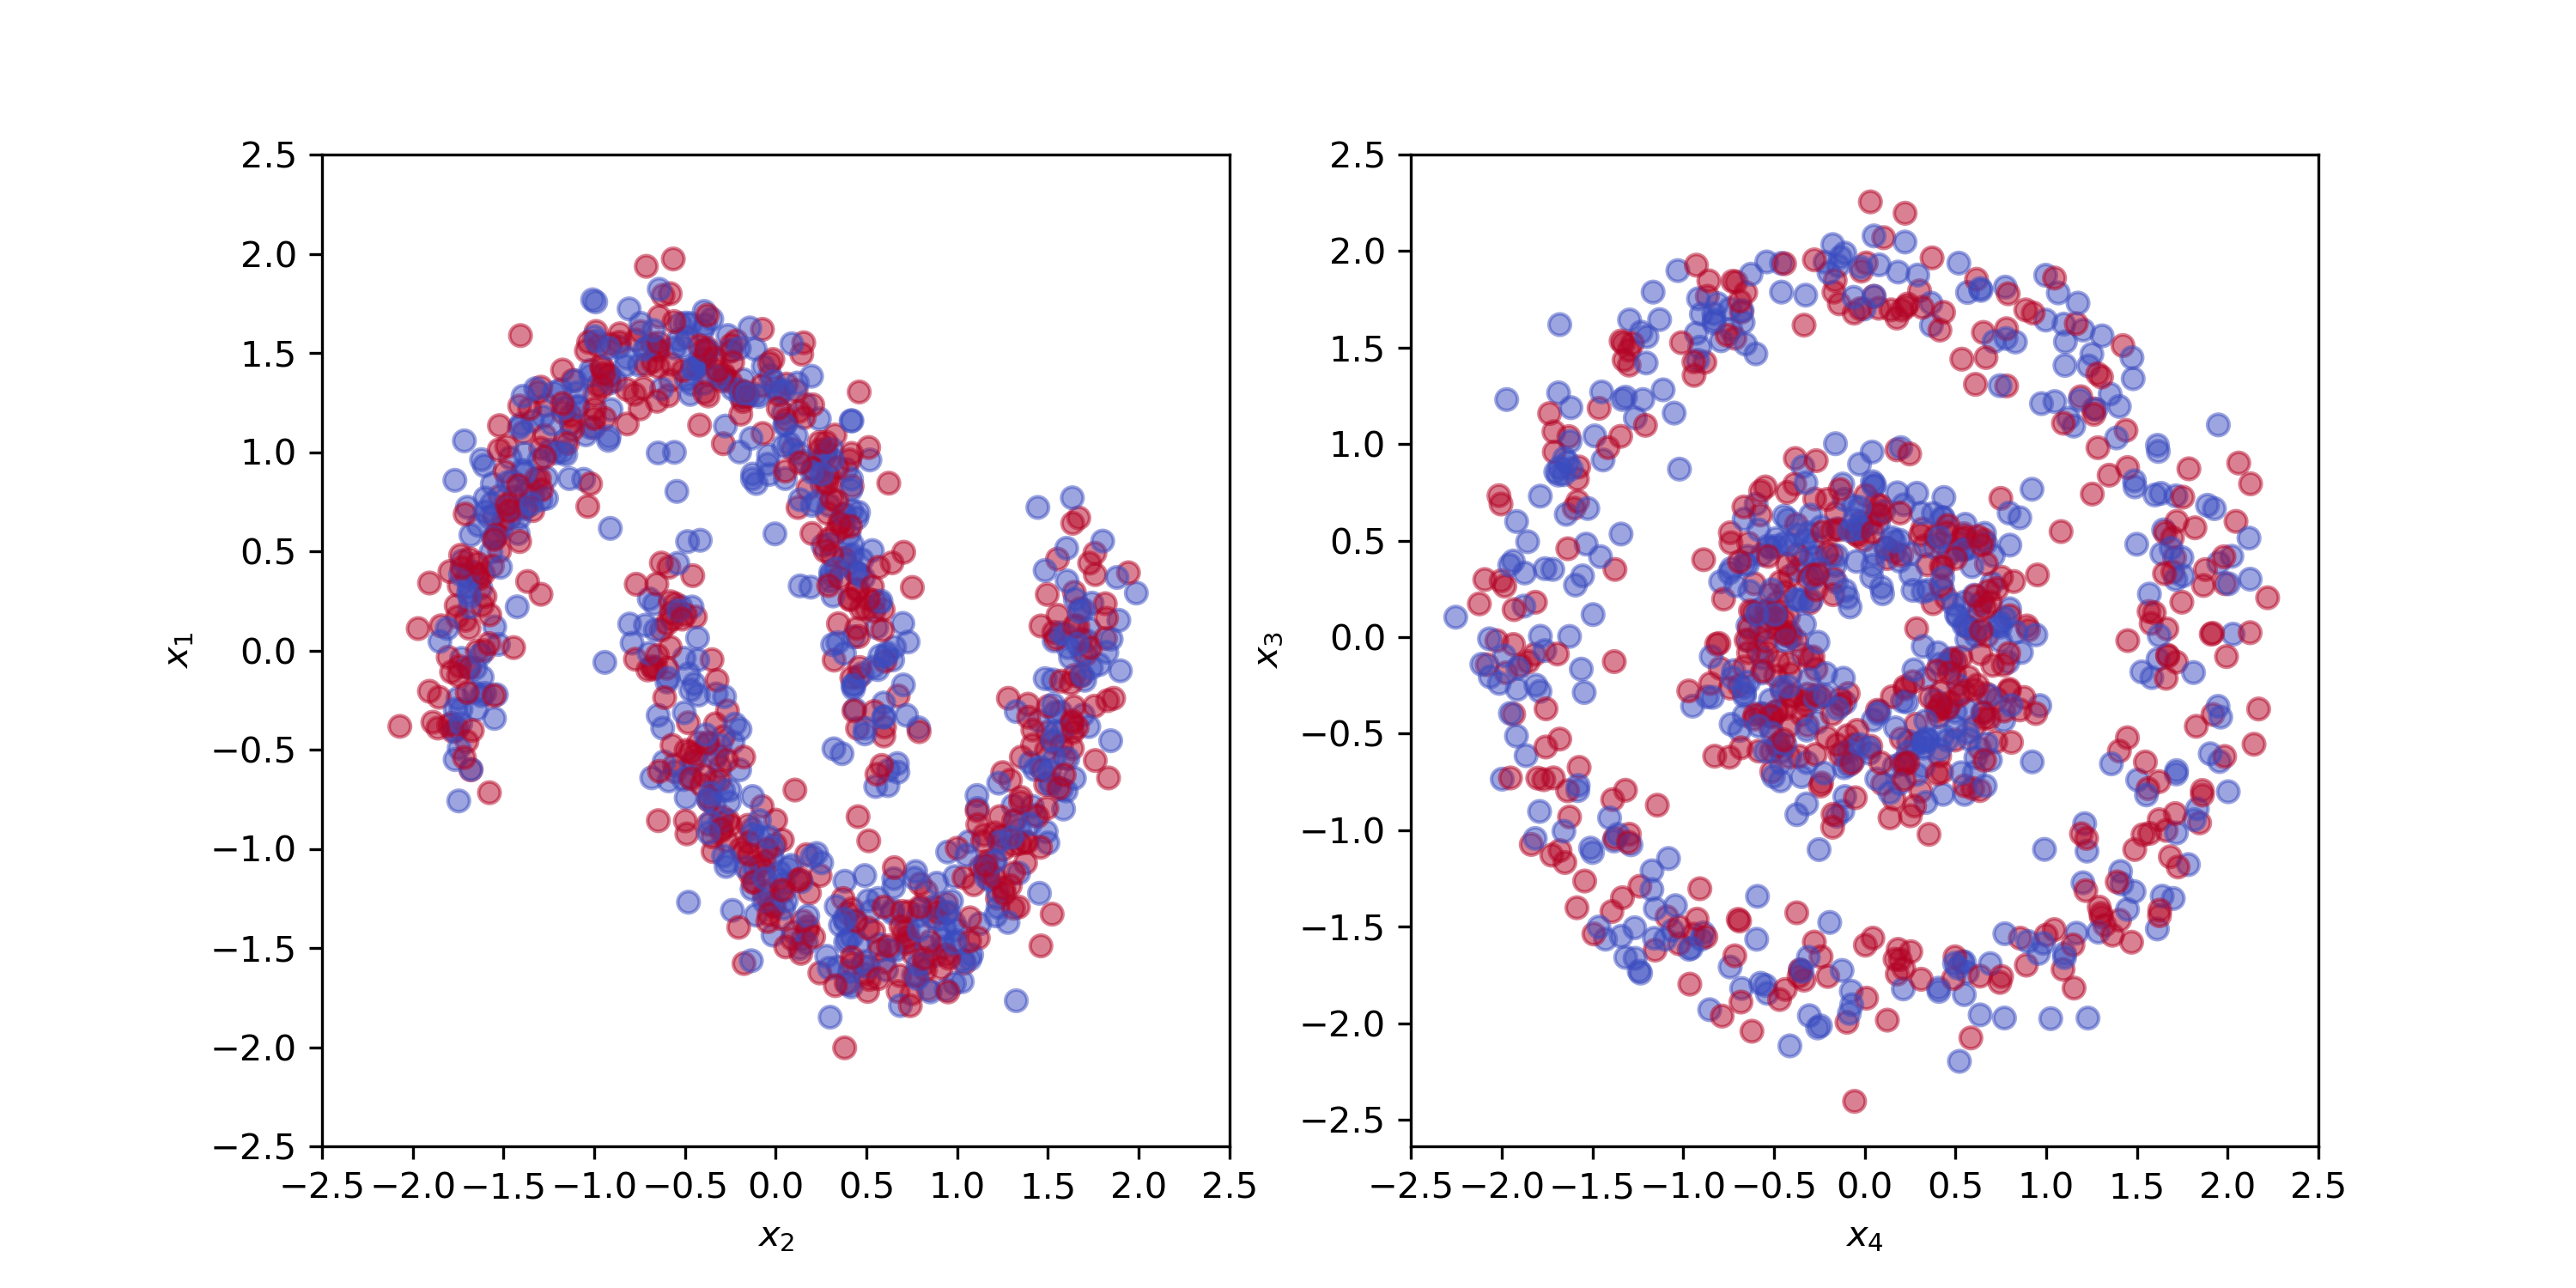
\includegraphics[width=1.0\linewidth]{moons-circles-inverted.png}
    \caption{
        This figure depicts the moons dataset on the left, where the colors are the labels of the circles dataset.
        On the right, the circles dataset is depicted, with the colors representing the class of the moons dataset.
    }\label{fig:moons_circles_inverted}
\end{figure}

This is demonstrated in figure~\ref{fig:moons_circles_inverted}.
The data is the exact same data as is visible in figure~\ref{fig:moons_circles}. 
However, one dataset is displayed with the labels of the other dataset and vice versa.
Concretely, on the left side, the coordinates represent $x_1$ and $x_2$, but the colors refer to $y_2$.
On the right side on the other hand, $x_2$ and $x3$ are displayed with the colors defined by $y_1$.
There is no clear visible pattern discernible from these dataset given on their own.

\section{The Network}
The neural network used to train on this task was inspired by the original lottery ticket experiments \autocite{DBLP:conf/iclr/FrankleC19}. 
A fully connected feed forward neural network was used.
The network has four input neurons, two output neurons and between one and three hidden layers.
Throughout the thesis, experiments with varying numbers of hidden layers are conducted.
The input neurons correspond to $x_1, x_2, x_3, x_4$ defined in the previous paragraph~\ref{sec:independece_dataset}.
The network outputs correspond to $y_1$ and $y_2$.

As non-linearity, the Rectified Linear Unit (ReLU) is used.
The gaussian Xavier-initialization~\textcite{XAVIER-GLOROT} was used by \textcite{DBLP:conf/iclr/FrankleC19} in the original experiments.
However, the authors did not justify their decision.
Since the networks use the ReLU activation function, gaussian Kaiming-initialization~\autocite{KAIMING-HE} will be used as the initialization technique.
The initialization of the biases is not mentioned by \textcite{DBLP:conf/iclr/FrankleC19}.
Throughout this thesis, biases of the network are initialized with zero.
The random initialization of the weights is explicitly controlled via a random seed, to enable reproducibility.
Throughout the thesis, experiments are repeated with three to five different seeds for more robust results.

For the Moons-Circles dataset, the binary cross entropy loss function is used.
It is calculated seperately for every output feature of the network.

\section{The Training Process}
With the dataset and architecture described above the aim was to find lottery tickets.
To accomplish this task, the classic Iterative Magnitude Pruning algorithm described in refIMP was employed used by \textcite{DBLP:conf/iclr/FrankleC19} in the original lottery ticket experiments.
The weights are rewound to $0$.
\textcite{LinearModeConnectivity} demostrated that the LeNet architecture trained on MNIST is stable at initialization, meaning that lottery can be found rewinding the weights to $t=0$ (the value at initialization). 
Since the model and dataset in our case is significantly less complex, it is assumed that the resetting the weights to zero is sufficient to discover lottery tickets.

As pruning criterion, the original magnitude pruning used by \autocite{DBLP:conf/iclr/FrankleC19} is used. 
Since \autocite{DBLP:conf/nips/ZhouLLY19} showed that magnitude pruning is amongst the best performing criteria, it was selected due to its simplicity and widespread usage.
Biases are not pruned.

Contrary to \autocite{DBLP:conf/iclr/FrankleC19} where layerwise pruning is applied, the network is pruned globally.
Concretely, the pruning criterion is applied to all weights at once.
This enables the algorithm to `select' the sparsity for each layer on it's own, resulting in less assumptions that have to be made.

One training run consists of $L$ pruning levels. 
At each pruning level, $p$-percent (pruning rate) of the remaining prunable parameters are set to zero.
The number of prunable parameters equals the number of weights that have not yet been pruned.
After $L$ pruning levels, the number of prunable parameters is termed the `pruning target'.

Over the pruning levels, the number of prunable parameters goes from the initial number to the pruning target.
The sequence of prunable paremters is termed `parameter trajectory'.
A parameter trajectory can be uniquely defined by 3 out of the following 4 values:
\begin{itemize}
    \item prunable parameters at initialization
    \item pruning levels
    \item pruning rate
    \item pruning target
\end{itemize}

Different combinations can be useful for different scenarios.

The networks are trained with the ADAM optimizer.
The learning rate is set to 0.001 and a batch size of 64 is used.
These values were selected based on their effectiveness in preliminary experiments. However it is important to note that they are somewhat arbitrary and may be suboptimal.
Further, throughout the experiments, early stopping is used to reduce the computational time.
Early stopping is implemented with a patience of 30 levels and the metric that is watched is the validation loss.
This means, if the validation does not improve for 30 consequtive epochs, the training of the level is stopped and the next level is started.

As a pruning target for the experiments with the Moons-Circles dataset, values between 100 and 120 were selected.
The pruning target is, in many experiments, derived from the model architecture which will be described in detail in a later chapter.
The pruning target refers to the number of unpruned weights after all pruning iterations are completed.
This however does not mean, that all the unpruned weights are of use to the network.
The number of active weights, which will be discussed in detail in this chapter, can be significantly lower than the pruning target.
It refers to the weights that actually influence the output of the network.

\begin{minipage}{\linewidth}
\begin{lstlisting}[language=Python,caption={This code snippet contains python-flavoured pseudo code.
    It depicts the general procedure of iterative magnitude pruning used for the experiments in this thesis.},captionpos=b, label={code:imp}]

    # given
    model: torch.nn.module  # the freshly initialized model 
    parameter_trajetory: List[int] # defines the pruning process
    train_data, test_data  # data for training
    
    # save state to reinitialze after pruning
    initial_model_state = save_model_state(model)
    
    parameter_count = parameter_trajetory[0]
    for target in parameter_trajectory:

        # no pruning before the first training
        if not first_iteration:

            # the number of parameters to prune from the model
            pruning_amount = parameter_count - parameter_target
            parameter_count = parameter_target

            # prune the model 
            prune(model, pruning_amount)

            # reinitialize the remaining values with initial values
            reinit(model, initial_model_state)

        # actual training and evaluation
        train_loss = train(model, train_data)
        val_loss, val_accuracy = evaluate(model, test_data)

        # transform to a graph and see if it split or degraded
        dag = transform_to_digraph(model)
        evaluate_dag(dag)

        # the run is stopped when graph is degraded 
        # to limit training time
        if graph_degraded:
            break

        # early stopping is used to limit training time
        if early_stopping:
            break
    \end{lstlisting}
\end{minipage}

In the code snippet~\ref{code:imp} the algorithm for iterative magnitude pruning is depicted in python-flavoured pseudo code.
Details have been omited for readability.
Imporantly, the order of the commands are outlined to give a better sense of the algorithm.
The algorithm requires a model, parameter trajectory and data.
The model refers to the freshly initialized neural network.
The parameter trajectory, as described earlier in this paragrah, refers to the number of weights the network should have at every pruning level.
The difference between two neighbouring entries in the parameter trajectory gives the number of parameters to prune in the given level.

\section{Network Splitting}
Since the goal of the experiments is to show if two seperate networks for inside the initial network, a mechanism to check if this is the case is needed.

Before the first pruning level, the network is converted into a Directed Acyclic Graph $\mathcal{G}$.
This graph representation is maintained throughout the pruning levels and updated after each level.

In the first step, each neuron is converted to a node in the graph.
Then each weight is converted into an edge that connects one node from the previous layer to the next layer.
All nodes, with the exception of the input layer, have biases associated with them.

Four categories are defined for the nodes and edges in the graph.
\begin{enumerate}
    \item active parameters  \\
    Nodes or edges in the graph that are connected to at least one input node and at least one output node.
    \item inactive parameters \\
    Nodes or edges that are not connected to any output node. They do not influence the result of the network and they do not receive gradients. They can be removed.
    \item pruned parameters \\
    Nodes or edges that have been masked out by the pruning algorithm.
    \item zombie parameters \\
    Nodes or edges that are not connected to any input node, but are connected to at least one output node.
\end{enumerate}
Before the first pruning level, all nodes and edges are classified as `active parameters'.
In the next step, each parameter in the graph will be assigned a category.
First, the newly pruned weights are extracted from the pytorch module.
Each edge in the graph that was pruned, is assigned that category.

Then, a subgraph $\mathcal{G}_{unpruned}$ is created, excluding all pruned weights.
On $\mathcal{G}_{unpruned}$, inactive nodes and edges are found and assigned their category.
All nodes that are not connected to any output node are classified as inactive.
Further, all edges that are connected to an inactive node are classified as inactive.

Then, a subgraph $\mathcal{G}_{active/zombies}$ is created, excluding all pruned and inactive weights.
On $\mathcal{G}_{active/zombies}$ zombie parameters are found and assigned to their category. 
All nodes that are not connected to any input feature are classified as a zombie parameter. 
Furhter, all edges that are connected to a zombie node are classified as a zombie parameter.

An active subgraph $\mathcal{G}_{active}$, where all nodes are connected to at least one input node and at least one output node.

\subsection{Matching Networks and Tasks}\label{sec:taskmatch}
The active graph $\mathcal{G}_{active}$ is used to find seperate components in the graph.
Conveniently, this can be done with a single networkx function.
\begin{lstlisting}[language=Python]
import networkx as nx

# G : nx.DiGraph
subnetworks = [
    G.subgraph(c) 
    for c in nx.connected_components(G.to_undirected())
]
\end{lstlisting}

Each node or edge of $\mathcal{G}_{active}$ is contained in exactly one of the subnetworks.
There is no overlap between the subnetworks.
Next, the subnetworks are matched to the tasks, which are defined by the dataset.
For each subnetwork and each task in the dataset, the inputs and outputs of the network are compared to the inputs and labels of the task.

Concretely, each task is associated with a set of inputs $T^{(i)}_{in}$ and a set of outputs $T^{(i)}_{out}$.
Further, each subnetwork contains a set of input nodes $N^{(j)}_{in}$ and a set output nodes $N^{(j)}_{out}$.

The intersection of the task inputs and the input nodes of the network denoted input coverage set $C^{(ij)}_{in}$ and output coverage set $C^{(ij)}_{out}$ for the outputs respectively.

\[
C^{(i,j)}_{out} = N^{(j)}_{out} \cap T^{(i)}_{out}
\]
\[
c^{(i,j)}_{out} = \frac{| C^{(i,j)}_{out} |}{|T^{(i)}_{out}|}
\]

\[
C^{(i,j)}_{in}  = N^{(j)}_{in}  \cap T^{(i)}_{in}
\]
\[
c^{(i,j)}_{in} = \frac{| C^{(i,j)}_{in} |}{|T^{(i)}_{in}|}
\]

For evaluating the coverage the the subnetworks as a whole, the number of paths from inputs to outputs are considered.
The total number of paths for a task is given by the product of the cardinatlity of the inputs set and the cardinality of the output set.
Similarly, the number of paths available in the subnetwork is given by the cardinality of theinput coverage set and the cardinatlity of the output coverage set.
The total coverage $c^{(i,j)}$ is defined as the ratio between the products.
\[
c^{(ij)} = \frac{
    | C^{(i,j)}_{in}| * | C^{(i,j)}_{out} |
    }{
    |T^{(i)}_{in}| * |T^{(i)}_{out}|
}
\]
The total coverage is 1 when the task is completely covered by the subnetwork.
It is 0, if either no input or no output of the task is covered by the subnetwork.
It is between 0 and 1, if at least one input and at least one output of the task is covered, but at least one input or output is not covered.
The total coverage is a useful indicator if all inputs and outputs are important, as they are counted equally.
In the case of the Moons-Circles Dataset, the total coverage is used.
For datasets where not all inputs or outputs are necessary or even desired to be used, the input coverage, output coverage or a combination thereof might be a more useful metric.

!!! Maybe move this to dataset.
!!! explain task description in dataset
!!! revise the math part. C is overloaded and number of tasks / subnetworks needs an identified. MAybe J, K and j, k for the running vars.

For instance, given the dataset in ref2, the dataset contains two tasks: the `moons'-task and the `circles'-task. 
The moons-task $T^{(1)}$ is associated with the inputs $T^{(1)}_{in} = \{x_1,x_2\}$ and the output $T^{(1)}_{out} = \{y_1\}$.
The circles-task $T^{(2)}$ is associated with the inputs $T^{(2)}_{in} = \{x_3,x_4\}$ and the output $T^{(1)}_{out} = \{y_4\}$.

The input, output or total coverage can be collected in a matrix $C$ of size $\tau \times j$, where $\tau$ is the number of tasks and $j$ the number of subnetworks. 
$c_{i,j}$ represents the value at the $i$-th row and the $j$-th column and $0 \leq c_{i,j} \leq 1$ holds.
Further, the sum of the matrix is upper bound by the number of tasks.
\[
\sum^{i} \sum^{j} c_{i,j} \leq \tau
\]


Given an unpruned network and a dataset with two tasks the matrix would look like the following 
\[
C = \begin{pmatrix}
    1 \\ 1
\end{pmatrix}
\]
Each task would be completely covered by the same network.
Since the network per definition covers all tasks before the first pruning level, the matrix will be a unit vector with as many entries as there are tasks.

After several pruning iterations, there network might contain two disconnected subnetworks.
In this case, an additional row is added to the matrix.
For instance, let the subnetworks perfectly match the tasks such that every task is completely covered by one subnetwork.
The matrix $C$ might look like the following.
\[
C = \begin{pmatrix}
    1 & 0 \\ 0 & 1
\end{pmatrix}
\]
After further pruning the network, all the connections to one of the input nodes might be pruned.
Then, one of the subnetworks would not be completely covered anymore.
Assuming there are one output node and two input nodes for task 1 and the subnetwork 2 covers all nodes except one input.
The resulting coverage would be 
\[
c^{(1,2)} =  \frac{
    | C^{(1,2)}_{in}| * | C^{(1,2)}_{out} |
    }{
    |T^{(1)}_{in}| * |T^{(1)}_{out}|
} = \frac{1}{2}
\]
and the resulting matrix $C$ would look like the following

\[
C = \begin{pmatrix}
    1 & 0 \\ 0 & 0.5
\end{pmatrix}
\]

If the sum of $C$ is equal to the number of tasks and the number of subnetworks is equal to the number of tasks, then the network is perfectly split.

If the sum of $C$ is equal to the number of task, but there are less subetworks than tasks, the network still needs to split.
The number of splits that are required can is the difference between the number of tasks and the number of subnetworks.

If the sum of $C$ is less than the number of tasks, the network already has lost at one input or output.
This scenario will be referred to as a `degraded' network.
Once a network is degraded, it is impossible that a perfect split is reached.
In the case of the Moons-Circles dataset, the training is stopped as soon as the network is degraded to save computational resources.

(additional)
For mnist, we use the output coverage, since it is expected that the network will come to ignore inputs.
Then the output coverage is used. Also between 0 and 1. Works the same way as with the total coverage in the previous case.

\section{Model Extension}
Model extension is a technique used to create models that are comparable on the basis of prunable parameters. 
First, the problem is described which model extension is intended to solve, then the technique is described in detail.
\subsection{The Problem}
To compare networks over different pruning levels, a significant quantity is the number of prunable parameters the networks has left at each iteration.
For instance, comparing two networks with 1000 and 1200 prunable parameters in the beginning, 6 pruning levels and a pruning rate of $0.2$, the following parameter trajectories $t_{1000}$ and $t_{1200}$ define the training.
\[
t_{1000} = [1000, 800, 640, 512, 409, 327, 262]
\]
\[
t_{1200} = [1200, 960, 768, 614, 491, 393, 314]
\]
Let $f_{1000}$ and $f_{1200}$ be the associated networks.
The first problem is that the pruning target is not aligned.
The final networks cannot be so easily compared, because they have different amounts of parameters available to them.
Therefore, let the pruning rate be variable. The pruning target set to the same value for both networks.
The pruning rate can be calculated with 
\[
p = 1 - \sqrt[L]{\frac{T}{P}}
\]
where $L$ is the number of pruning levels, $P$ equals the number of prunable parameters before pruning and $T$ denotes the pruning target.

Let the pruning target be $200$ with 6 pruning levels.
The pruning rates are $p_{1000} = 0.235$ and $p_{1200} = 0.258$ respectively.
The resulting parameter trajectories are as follows.
\[
t_{1000} = [1000, 764, 584, 447, 341, 261, 200]
\]
\[
t_{1200} = [1200, 890, 660, 489, 363, 269, 200]
\]

With this change, the pruning targets are aligned and therefore, the final networks are comparable in a more fair way.
However, the number of available parameters is \textit{only} aligned at the very end.
Consider the follwing situation.
The network $f_{1000}$ seperates after the fourth pruning level, where it has $341$ prunable parameters left. 
The other network $f_{1200}$ seperates at iteration after the fifth level, where it has $269$.
At first glance, one could say that the network $f_{1000}$ seperated earlier.
It seperated when it had more parameters available than the other network.
However, this misses part of the picture.
Given that the networks can only seperate at the predefined trajectory, the network $f_{1200}$ would have had to seperate at $363$ parameters.
Therefore, the $f_{1200}$ \textit{maybe would} seperate earlier than $f_{1000}$.
In the range of $363$ to $341$ where the $f_{1200}$ would have more parameters than $f_{1000}$, is not checked anymore.
This makes it hard to compare the networks during their pruning trajectory.
Especially regariding the pruning level when they split, as they cannot be compared fairly.

Ideally, different networks would have parameter trajectory that are shared, such that they can be compared at every step.
To achieve this on can `extend the model'.

\subsection{The Solution}
The objective is to create networks, that share the parameter trajectory.
To achieve this, we will starts with a small network which will be referred to as the base model.
Let the base model be a network with the shape $(4, 8, 8, 2)$.
This network has $112$ weights and $18$ biases.
To extend this network, a pruning rate $p$ must be defined.
The task now is to find a larger network, which will have the same number of unpruned parameters \textit{after} it was pruned with the defined pruning rate.

To extend the model now for one level, a new architecture has to be found, which, when pruned once with a pruning rate of $p=0.32$, has $112$ remaining parameters.
To extend the base model for two levels, the same method is used, but the resulting network must be pruned twice to reach the desired number of parameters, $112$ in this case.
To keep the task simple, the network architecture is restricted to a fixed number of hidden layers where each layer contains the same number of neurons.
Further, for the experiments in this thesis, only the weights are considered, since biases are not pruned.
However, the technique is easily extensible to take the biases into account.

Concretely, let $N$ be the number of weights in a network.
The equation to calculate the number of weights is given as follows

\begin{equation} \label{eq:num_params}
    d_h d_{in}+(m-1)d_h^2 + d_h d_{out} = N
\end{equation}

, where $d_{in}$ and $d_{out}$ refer to the input and output dimension respectively, $m$ to the number of hidden layers and
$d_h$ to the number of neurons per hidden layer.
For the base model with shape $(4, 8, 8, 2)$ the values are $d_h=8$, 
$d_{in}=4$, $d_{out}=2$ and $m=2$.
 
To extend the model with a given pruning rate $p=0.32$, the number of parameters is updated to a target value denoted $\hat N$.
The value $\hat N$ should have the property that, when pruned with a pruning rate of $p$, it should again be $N$.

Therefore, for one extension level:
\[
\hat N = {(\frac{N}{1-p})}
\]
And generalising for any number of extension levels

\[
\hat N = {\frac{N}{{(1-p)}^L}}
\]
,where $L$ refers to the number of extension levels.

$\hat N$ now represents the target number of parameters. 
To find a network architecture that has this amount of parameters, one needs to insert $\hat N$ in the equation~\ref{eq:num_params}.
All parameters except for $d_h$ are set to a fixed value and the equation is solved for $d_h$.
Equation~\ref{eq:num_params} can be reformulated to a standard quadratic equation.

\[
    (m-1)d_h^2 + (d_{out} + d_{in}) d_h - \hat N = 0
\]
and therefore solved for $d_h$ with 
\[
    d_h = \frac{
        - d_{out} - d_{in} \pm \sqrt{  {(d_{out} + d_{in})}^2 + 4 \hat N (m-1) } 
    }{
        2(m-1)
    }
\]

The result of $d_h$ refers to the target number of hidden neurons in each layer.
However, it most likely is not an integer directly.
Therefore, the value is simply rounded to the nearest integer.

In the case of the network with $112$ weights and a pruning rate of $0.32$, $\hat N$ evaluates to $164.706$.
Entering $\hat N$ into the equation and solving for $d_h$, the two solutions are $d_h=10.1795$ and $d_h=-16.1795$.
Only positive solutions are of interest, therefore the second solution can be omitted.
Rounded to the nearest integer, the number of hidden neurons in each layer is set to $10$.

Through rounding the pruning rate is slightly different at every iteration.
This is generally the case when a pruning rate is given as a percentage, since the number of weights that are actually pruned are always discrete.
In the previous example, the actual pruning rate would be calculated as follows:
The number of weights for the architecture extended by one level, would be $160$.
The effective pruning rate is therefore $p_{eff}=1-\frac{112}{160}=0.3$.

A network can be extended an arbitrary number of times.
Importantly, the number of weights are fixed for each extension level.
The number of weights a network has at level one does not change, independent of the number of total extension levels.
Therefore, the networks share the same parameter trajectory as long as they are extended from the same base model with the same pruning rate.
This enables comparing networks of different sizes throughout all pruning levels they share.

\section{The MNIST-Fashion-MNIST Dataset}\label{sec:mnist}
To test the network splitting on a slightly more realistic problem, the MNIST-Fashion-MNIST dataset was created.
This dataset is created in the same way as described in paragraph~\ref{sec:independece_dataset}.
But contrary to the toy datasets used from the previous chapter, the MNIST dataset \autocite{mnist} and the fashion-mnist \autocite{fashion}.
The MNIST dataset is a well known dataset of handwritten digits. 
The training set consists of 60000 images and the test set of 10000.
It contains all digits from zero to nine in hanwritten form, on a $28 \times 28$ pixel grayscale image.
This dataset was also used in the experiments original lottery ticket experiments \autocite{DBLP:conf/iclr/FrankleC19}.

\begin{figure}[ht]
    \centering
    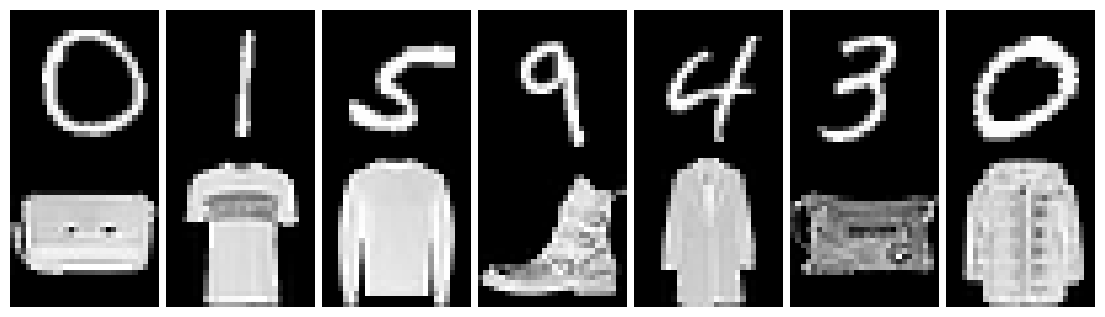
\includegraphics[width=1.0\linewidth]{mnist-fashion-mnist.png}
    \caption{
        This figure depicts the mnist-fasion-mnist dataset. 
        Seven randomly selected samples are displayed next to each other.
        On top of each image, the handwritten digit is displayed. 
        On the bottom, the fashion item.
        Each sample consists of one random digit and one random fashion item.
    }\label{fig:mnist_fashion}
\end{figure}

As the name suggests, the fashion-MNIST dataset \autocite{fashion} is similar to the MNIST dataset.
However, instead of handwritten digits, different items of clothing are displayed on the $28 \times 28$ grayscale image.
It contains the same number of images for the test set and the training set.
Both datasets contain 10 classes.

In the same way as described in paragraph~\ref{sec:independece_dataset}, the datasets are concatenated into one.
Both datasets are shuffled and each sample from the MNIST dataset is concatenated with a random sample from the Fashion-MNIST dataset.
The class labels are also concatenated.

The result is a dataset with 60000 training samples and 1000 evaluation samples.
Through the concatenation, each image has an aspect ratio of $28 \times 56$, where each half corresponds to one of the datasets.

Contrary to the previous task, this dataset contains significantly more input features.
Each dataset has 784 input features, which results in 1586 input features for the concatenated dataset.
Further, the previous task was a combination of two binary classification tasks.
Now, each dataset represents a multiclass classification problem with 10 classes.

\subsubsection{Loss Function}
To enable training with this dataset, the loss has to adapted.
For classification with more than two classes, the categorical cross entropy can be used.
For each of the tasks in the concatenated dataset the loss is computed seperately.
The total loss is simply the sum of the losses from each task.

Concretely, let $\mathbf{\hat y_{mnist}} = \left[\hat y_1, \dots, \hat y_{10}\right]$ be the output logits of the network that relate to the MNIST datset and $\mathbf{\hat y_{fashion}} = \left[\hat y_{11}, \dots, \hat y_{20}\right]$ to the Fashion-MNIST dataset.
The labels are denoted fashion $\mathbf{y_{mnist}}$ and $\mathbf{y_{fashion}}$ respectively.
Together, the form the network output $\mathbf{\hat y} = \left[\hat y_1, \dots, \hat y_{20}\right]$

Let, $\mathcal{L} (\mathbf{\hat y}, \mathbf{y})$ be the loss of the network output and the true labels $\mathbf{y}$.

The total loss of the network $\mathcal{L}$ is calculated as follows:

\[
\mathcal{L}  (\mathbf{\hat y}, \mathbf{y})
= \ell  (\mathbf{\hat y_{mnist}}, \mathbf{y_{mnist}})
+ \ell (\mathbf{\hat y_{fashion}}, \mathbf{y_{fashion}})
\]

,where $\ell$ represents the categorical cross entropy loss.

\subsubsection{Adapting Network Degradation}
Previously, network seperation and network degradation was introduced.
When trained on the Moons-Circles dataset from paragraph~\ref{sec:independece_dataset}, a network counts as degraded when any of the inputs or outputs are cut off from the network, since all inputs and outputs are relevant for the networks success.
However, regarding the MNIST-Fashion-MNIST dataset, this is not the case.
Many of the input features do not carry information, for example the outer frame of the MNIST images.
Therefore, it is to be expected that all connections to these inputs may be pruned.
This would likely lead to unwanted network degradation.

Therefore, the network only counts as degraded, if an output neuron is completely cut off.
This requires only a small change in the calculation of the coverage as shown in paragraph~\ref{sec:taskmatch}.
The terms relating to the inputs of the tasks, namely $C_{in}$ and $T_{in}$, are simply to be exchanged for one.